\label{sec:singular1}

Considere a minimização da seguinte função objetivo:
%
\begin{equation}
	\label{eq:singular1:J}
	J = x_3(t_f)
\end{equation}
%
sujeito ao seguinte sistema de equações diferenciais ordinárias, bem como uma restrição para o controle:
%
\begin{equation}
	\label{eq:singular1:dinamica}
	\begin{gathered}
		\dot{x}_1(t) = x_2(t), \;\; x_1(0) = 0\\
		\dot{x}_2(t) = u(t), \;\; x_2(0) = 1 \\
		\dot{x}_3(t) = x_1^2(t), \;\; x_3(0) = 0\\
		-1 \leq |u(t)| \leq 1
	\end{gathered}
\end{equation}
%
em que $t$ é o tempo ($t_f$ é o tempo final) e $\mathbf{x}(t) = \begin{bmatrix} x_1(t) & x_2(t) & x_3(t) \end{bmatrix}^T $ é o vetor de variáveis de estado e $ u(t) $ a variável de controle. 

Conforme comentado para o primeiro exemplo, a estimativa inicial para os perfis de estado e controle foi inicializada de forma \textit{default} por cada um dos pacotes. \textcolor{red}{Arthur, aqui já devemos ter apresentado a metodologia usada por cada pacote para definir o chute. Isto deve ser feito na apresentação de cada um dos pacotes, respectivamente (na revisão bibliográfica e na metodologia, respectivamente.)}

Na Figura \ref{fig:singular1:sensibilidade:J} são apresentadas a influência do melhor valor da função objetivo encontrada $ J^* $ em relação ao número de nós utilizados. Também foi determinado o número mínimo de nós de colocação ($ N_m $) necessários para a convergência do resultado para a solução reportada na literatura. Cabe ressaltar que foram escolhidos 30 valores igualmente espaçados dentro do intervalo [5 150]. 

De forma geral observa-se que, para cada um dos pacotes analisados, a partir de um número mínimo de nós de colocação, sempre foi possível encontrar a solução reportada na literatura, a saber, $ J^* $= \textcolor{red}{Arthur, qual o valor??? coloque a referência base}. Ressalta-se que, empregando os métodos $ PSOPT_t $ ou $ PSOPT_h $, não foi possível determinar a solução para pequenos valores para $N$ (entre 5 e 50, aproximadamente). Além disso, destaca-se que, no caso do $ COPILOTS_h $, optou-se por atribuir a $ N_m $ o $ N $ associado ao menor valor de $ J^* $, uma vez que, após atingir esse valor, o custo ótimo passou a crescer antes de alcançar a convergência. 

Os valores de $ J^* $ associados aos resultados obtidos usando o $ COPILOTS_h $ convergiram rapidamente, o que se deve ao SQP e às características numéricas inerentes à colocação Hermite-Simpson, isto é; maior precisão. Em contrapartida, os valores de $ J^* $ associados ao $ PSOPT_l $ apresentaram uma convergência mais lenta do que aquela observada nos demais métodos. Esse comportamento pode ser justificado pelas propriedades numéricas da colocação pseudo-espectral, cujo emprego na resolução de PCOs que apresentam descontinuidades nos controles não é recomenda \cite{becerra_tutorial_2010}.

Os resultados obtidos pelo $ FALCON $ e pelo $ COPILOTS_t $ se mostraram bem próximos, uma vez que ambos utilizam a colocação trapezoidal. Cabe ressaltar que, nesses casos, foi possível solucionar o PCO mesmo para valores de $ N $ pequenos, algo que não foi possível  utilizando-se o $ PSOPT_t $, que também emprega a colocação trapezoidal. 

\noindent	
\begin{minipage}{\textwidth}
	\vspace{\onelineskip}
	\centering
	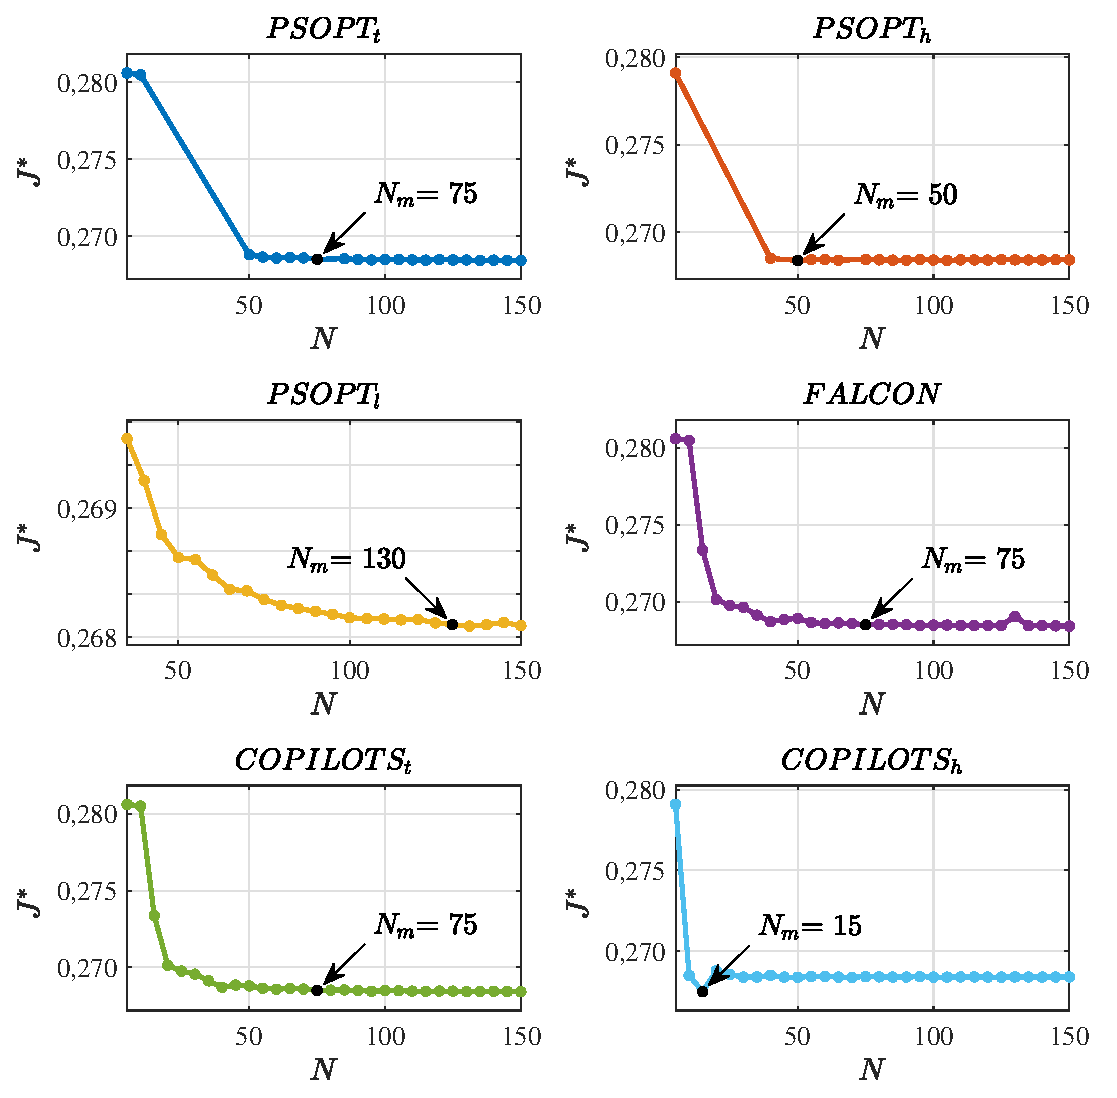
\includegraphics[scale=0.7]{fig/resultados/singular1/sens/J}
	\captionof{figure}[Influência do número de nós de colocação no valor da função objetivo para o problema singular 1]{Influência do número de nós de colocação $ N $ no valor da função objetivo $ J^* $ para o problema singular 1.}
	\label{fig:singular1:sensibilidade:J}
	\vspace{\onelineskip}
\end{minipage}

A Tabela \ref{tab:singular1:raw} apresenta as métricas obtidas por cada um dos pacotes considerando $ N = N_m $. Como destacado no primeiro estudo de caso, $ J^* $ é o valor da função objetivo, $ t_p $ é o  tempo de processamento médio, $ s_t $ é o desvio padrão com relação à  $ t_p $, $ n_{aval} $ é o número de avaliações da função objetivo, $ \Delta c_{max} $ é a máxima violação das restrições, $ N_s $ é o número de execuções bem sucedidas.

\begin{table}
	\centering
	\caption[Métricas obtidas para o problema singular 1]{Métricas obtidas para o problema singular 1. Os melhores valores para $ N_m $, $ J^* $, $ t_p $, $ n_{aval} $ e $ N_s\% $ encontram-se destacados.}
	\label{tab:singular1:raw}
	\begin{tabular}{@{}ccccccccc@{}}
		\toprule
		Método       & $N_m$                              & $J^*$                                   & $t_p$ {[}$s${]}                         & $s_t$ {[}$s${]} & $n_{aval}$                         & $\Delta c_{max}$                         & $N_s$ & $N_s\%$                                  \\ \midrule
		$PSOPT_t$    & 75                                 & 0,26850                                 & 16,30566                                & 0,26206         & 6140                               & 4,44e-12                                 & 22    & 73,33\%                                  \\
		$PSOPT_h$    & 50                                 & 0,26838                                 & 3,28051                                 & 0,18163         & 951                                & 1,99e-07                                 & 22    & 73,33\%                                  \\
		$PSOPT_l$    & 130                                & 0,26846                                 & 29,17814                                & 1,97563         & 429                                & 3,77e-08                                 & 24    & 80,00\%                                  \\
		$FALCON$     & 75                                 & 0,26851                                 & {\color[HTML]{009901} \textbf{0,23411}} & 0,04632         & {\color[HTML]{009901} \textbf{49}} & 5,62e-08                                 & 30    & {\color[HTML]{009901} \textbf{100,00\%}} \\
		$COPILOTS_t$ & 75                                 & 0,26850                                 & 22,39840                                & 0,50176         & 61812                              & 1,02e-09                                 & 30    & {\color[HTML]{009901} \textbf{100,00\%}} \\
		$COPILOTS_h$ & {\color[HTML]{009901} \textbf{15}} & {\color[HTML]{009901} \textbf{0,26749}} & 3,43669                                 & 0,05187         & 16303                              & 3,82e-13 & 30    & {\color[HTML]{009901} \textbf{100,00\%}} \\ \bottomrule
	\end{tabular}
\end{table}

Primeiramente, nota-se nesta tabela que foi necessário um número maior de nós de colocação utilizando-se métodos que fazem uso da colocação trapezoidal ($ PSOPT_t $, $ FALCON $ e $ COPILOTS_t $) em comparação com aqueles que utilizam a colocação Hermite-Simpson. Essa diferença se deve às características numéricas inerentes a cada método. Além disso, observa-se que os valores de $ J^* $ relacionados às soluções obtidas empregando colocação trapezoidal são bastante próximos uns dos outros, enquanto os valores de $ N_m $ a elas associadas são iguais.

O maior valor de $ N_m $ está associado ao $ PSOPT_l $, sendo esse outro indício de que a colocação pseudo-espectral não deve ser empregada na solução de problemas singulares. Aos métodos que utilizam a colocação Hermite-Simpson associam-se os menores valores de $ N_m $, devido às características numéricas inerentes a esse tipo de colocação. O menor valor de $ N_m $ está associado ao $ COPILOTS_h $, provavelmente, por conta do uso que o pacote faz do SQP. Ainda assim, apesar do baixo número de nós de colocação associado ao resultado obtido por meio desse pacote, é a ele que se atribui o menor $ J^* $. 

Ao $ FANCON $ estão associados o menor $ t_p $ e o menor $ n_{aval} $, apesar do $ N_m $ a ele atribuído ter sido maior do que os associados ao $ PSOPT_t $ e ao $ COPILOTS_h $. Esse comportamento se deve, mais uma vez, ao uso que o $ FALCON $ faz de ferramentas simbólicas na obtenção de derivadas analíticas. Os maiores $ t_p $ foram obtidos pelo $ PSOPT_l $ devido ao elevado valor do parâmetro $ N_m $ associado a esse pacote, e ao $ COPILOTS_t $ devido ao uso que o $ COPILOTS $ faz do SQP e às características numéricas inerentes a colocação trapezoidal. Pelas mesmas razões, a utilização do $ COPILOTS $, independentemente do tipo de colocação considerado, está associada a valores de $ n_{aval} $ consideravelmente altos, em comparação com os demais métodos avaliados. Observa-se que nem sempre $ t_p $ está diretamente relacionado ao $ n_{aval} $. Por exemplo, o tempo de processamento associado ao $ PSOPT_t $ é menor que o atribuído ao $ PSOPT_l $. O mesmo pode ser observado em relação ao $ N_m $ e $ n_{aval} $. Ressalta-se ainda que o $ COPILOTS $ e o $ FALCON $ possibilitaram a resolução do problema analisado para qualquer um dos valores de $ N $ adotados. 

Os perfis referente as variáveis de estado e de controle considerando $ N = N_m $ são apresentadas nas Figuras \ref{fig:singular1:x:x1} à  \ref{fig:singular1:u:u}. De forma geral, constata-se que os perfis obtidos por cada um dos pacotes é similar, apesar das leves oscilações observadas nas trajetórias de $ x_1(t) $ e $ x_2(t) $ advindas do emprego do $ PSOPT_l $. 

\noindent
\begin{minipage}{\textwidth}
	\vspace{\onelineskip}
	\centering
	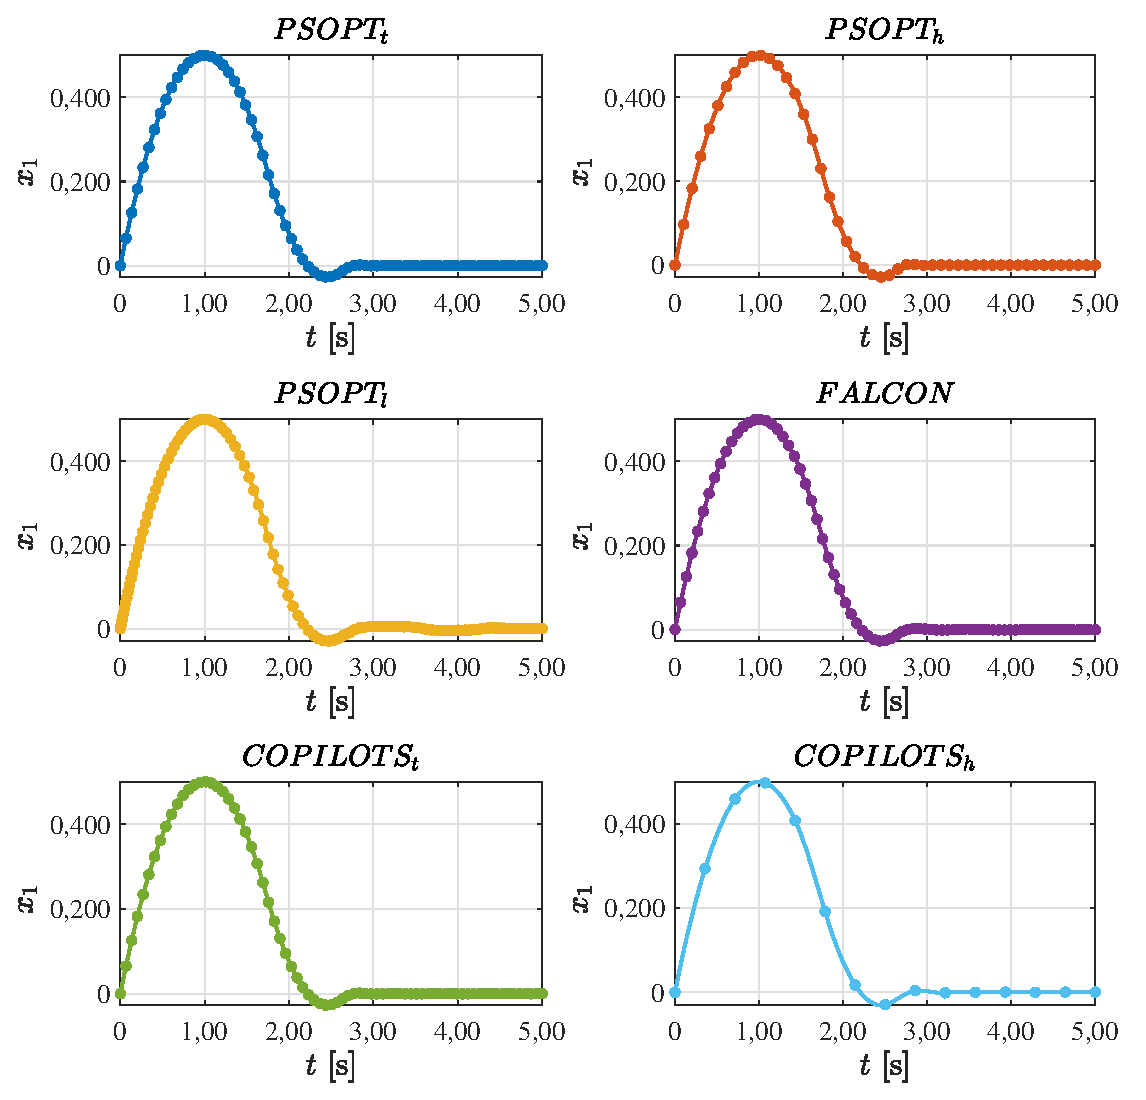
\includegraphics[scale=0.7]{fig/resultados/singular1/traj/x/x_1}
	\captionof{figure}[Variável de estado $x_1(t)$ para o problema singular 1]{Variável de estado $x_1(t)$ para o problema singular 1. Os pontos representam os valores discretizados e as linhas contínuas representam as trajetórias interpoladas.}
	\label{fig:singular1:x:x1}
	\vspace{\onelineskip}
\end{minipage}

Com relação as trajetórias de controle pode-se observar que estas apresentam a mesma tendência, apesar de diferenças em cada um dos pacotes utilizados. Primeiramente, verificam-se descontinuidades nos controles,  em $ t \approx 1,75 \, s $ e $ t \approx 2,5 \, s $, que são inerentes à solução do estudo de caso em análise. Além disso, nota-se que a presença dessas descontinuidades leva ao aparecimento de oscilações nos controles. Dentre as trajetórias de controle obtidas, a mais oscilatória é aquela advinda do emprego do $ PSOPT_l $, o que se deve ao alto $ N_m $ utilizado e às limitações numéricas inerentes à colocação trapezoidal. De fato, leves oscilações podem ser verificadas em todas as trajetórias, principalmente naquelas associadas ao $ PSOPT_t $ e ao $ COPILOTS_t $. Porém, apesar de também empregar a colocação trapezoidal, o $ FALCON $ foi o pacote que possibilitou a obtenção da trajetória mais suave. Tal comportamento pode ser justificado pela precisão dos resultados ao se empregar  ferramentas simbólicas na obtenção de derivadas.

\noindent
\begin{minipage}{\textwidth}
	\vspace{\onelineskip}
	\centering
	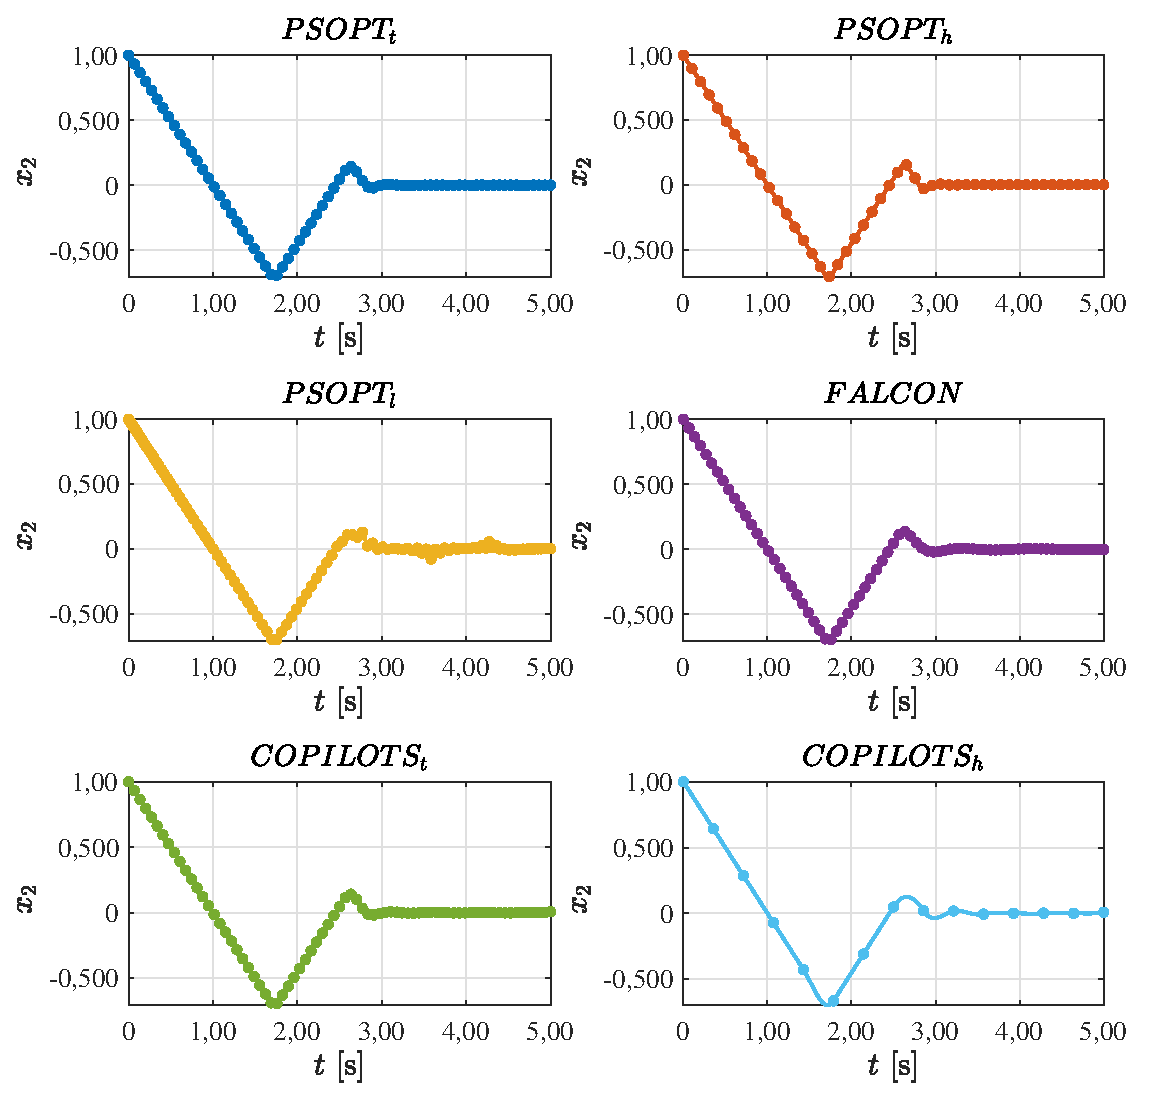
\includegraphics[scale=0.7]{fig/resultados/singular1/traj/x/x_2}
	\captionof{figure}[Variável de estado $x_2(t)$ para o problema singular 1]{Variável de estado $x_2(t)$ para o problema singular 1. Os pontos representam os valores discretizados e as linhas contínuas representam as trajetórias interpoladas.}
	\label{fig:singular1:x:x2}
	\vspace{\onelineskip}
\end{minipage}

Por fim, ressalta-se que as trajetórias de controle interpoladas considerando o $ COPILOTS_h $ e o $ PSOPT_l $, em alguns pontos, desrespeitam as restrições de caminho associadas ao estudo de caso em análise, que impõe que $ -1 \leq u(t) \leq 1 $. Além disso, nota-se o aparecimento de descontinuidades na trajetória atribuída ao $ COPILOTS_h $, em $ t = 2,85 \, s $ e $ t = 3,57 \, s $. Esse comportamento se deve ao tipo de interpolação associada à colocação Hermite-Simpson.

Foi também verificado a influência do aumento no número de nós de colocação tem no tempo de processamento e no número de avaliações da função objetivo, conforme as Figuras \ref{fig:singular1:sensibilidade:t} e  \ref{fig:singular1:sensibilidade:naval}. Nestes gráficos são apresentadas as variações: $ \Delta t_p = \max\{t_p\} - \min\{t_p\} $ e $ \Delta n_{aval} = \max\{n_{aval}\} - \min\{n_{aval}\} $. Os pontos nos gráficos representam os valores atribuídos a $ t_p $ (e a $ n_{aval} $) para cada um dos $ N $ considerados, enquanto as linhas contínuas representam curvas de tendência, obtidas por meio de regressões lineares, em que $R^2$ é o coeficiente de determinação. Os valores de $ N $ empregados na geração desses resultados são iguais àqueles considerados na computação da relação entre $ J^* $ e $ N $. 


\noindent
\begin{minipage}{\textwidth}
	\vspace{\onelineskip}
	\centering
	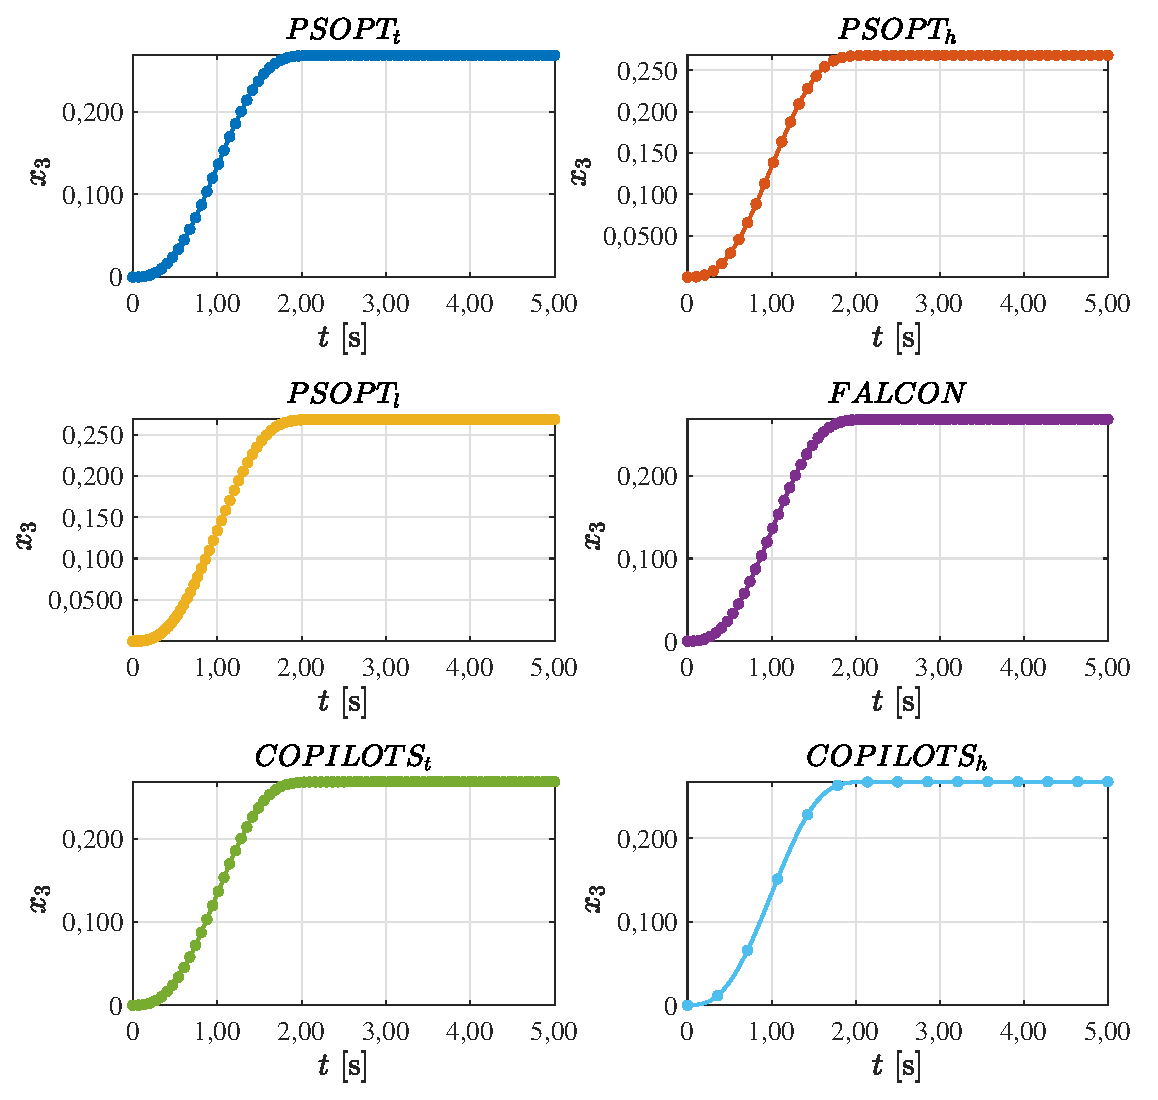
\includegraphics[scale=0.7]{fig/resultados/singular1/traj/x/x_3}
	\captionof{figure}[Variável de estado $x_3(t)$ para o problema singular 1]{Variável de estado $x_3(t)$ para o problema singular 1. Os pontos representam os valores discretizados e as linhas contínuas representam as trajetórias interpoladas.}
	\label{fig:singular1:x:x3}
	\vspace{\onelineskip}
\end{minipage}

Primeiramente, avaliando os resultados obtidos pelo $ COPILOTS $ verifica-se uma relação quadrática entre $ t_p $ e $ N $, e entre $ n_{aval} $ e $ N $. Neste caso, os elevados valores de $ n_{aval} $ e $ t_p $ pode ser justificados pela metodologia empregada para resolver o PPNL. Por outro lado, os resultados indicam que o $ FALCON $ é o método menos sensível a variações em $ N $, uma vez que, a partir do seu emprego, verificaram-se os menores valores de $ \Delta t_p $ e $ \Delta n_{aval} $ em comparação com os demais métodos em análise. Observa-se ainda que os $ t_p $ associados ao $ PSOPT_l $ são mais sensíveis ao aumento de $ N $ que aqueles atribuídos ao $ PSOPT_t $ e ao $ PSOPT_h $, considerando-se o alto $ \Delta t_p $ associado ao $ PSOPT_l $. No entanto, observou-se que o inverso é válido quando analisada a sensibilidade de $ n_{aval} $, tendo em vista o baixo $ \Delta n_{aval} $ atribuído ao $ PSOPT_l $ em comparação com aqueles associados ao $ PSOPT_t $ e ao $ PSOPT_h $.

\noindent
\begin{minipage}{\textwidth}
	\vspace{\onelineskip}
	\centering
	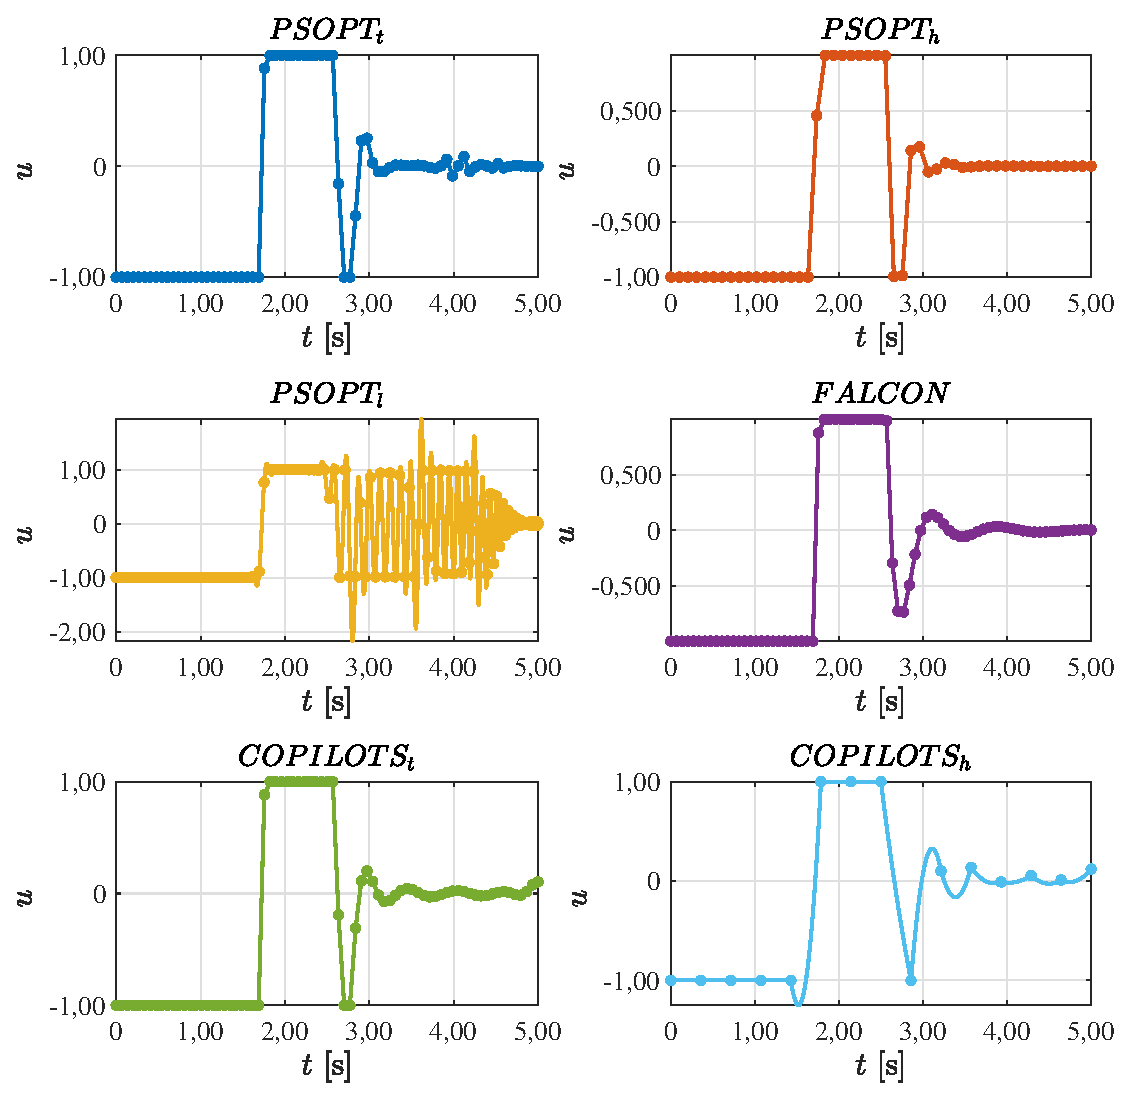
\includegraphics[scale=0.7]{fig/resultados/singular1/traj/u/u}
	\captionof{figure}[Variável de estado $u(t)$ para o problema singular 1]{Variável de estado $u(t)$ para o problema singular 1. Os pontos representam os valores discretizados e as linhas contínuas representam as trajetórias interpoladas.}
	\label{fig:singular1:u:u}
	\vspace{\onelineskip}
\end{minipage}

\noindent
\begin{minipage}{\textwidth}
	\vspace{\onelineskip}
	\centering
	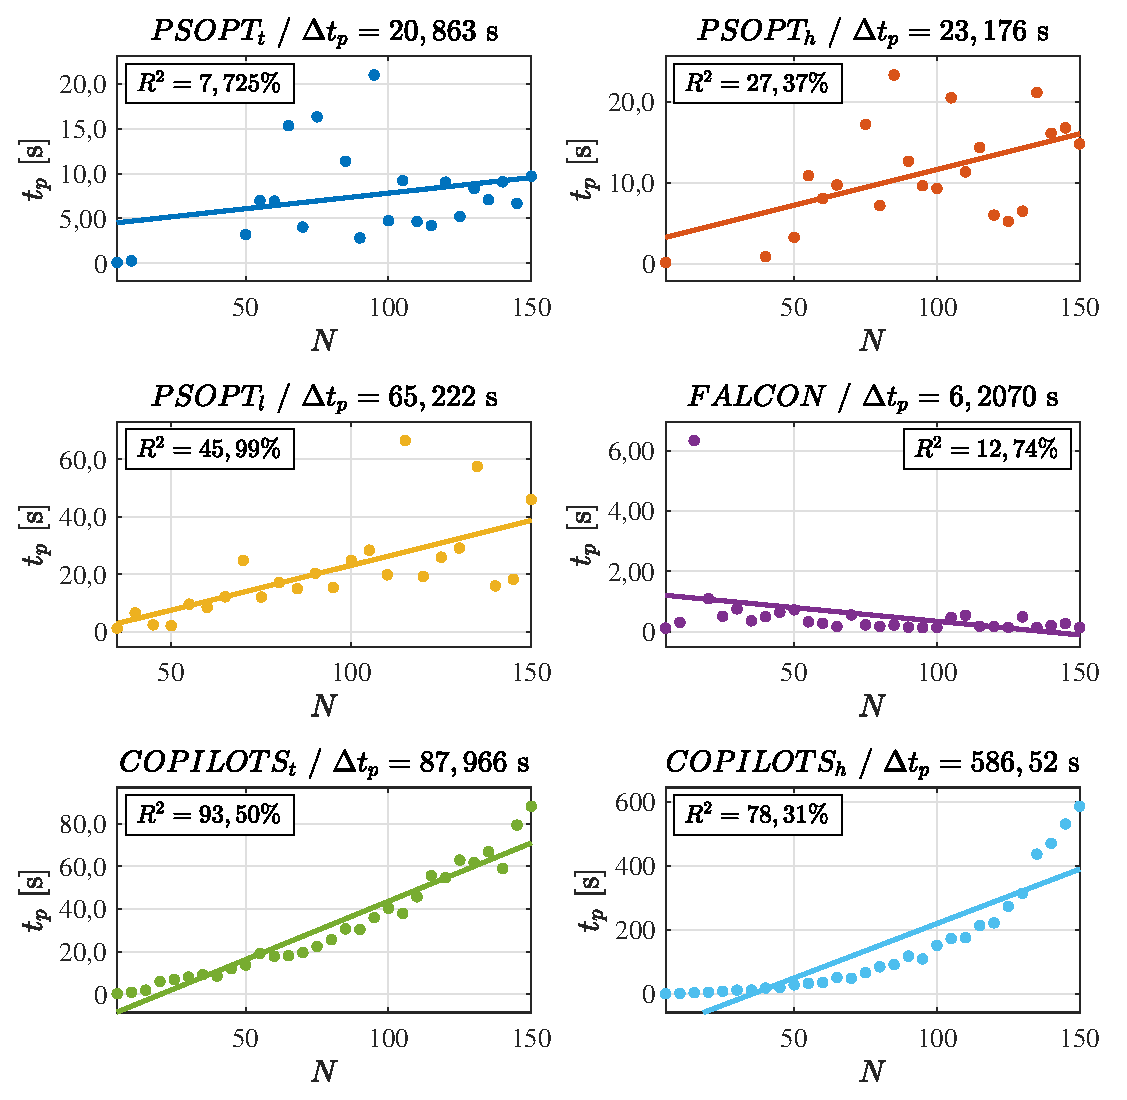
\includegraphics[scale=0.7]{fig/resultados/singular1/sens/t}
	\captionof{figure}[Relação entre o tempo de processamento e o número de nós de colocação para o problema singular 1]{Relação entre o tempo de processamento $ t_p $ e o número de nós de colocação $ N $, considerando cada um dos métodos em análise.}
	\label{fig:singular1:sensibilidade:t}
	\vspace{\onelineskip}
\end{minipage}

\noindent
\begin{minipage}{\textwidth}
	\vspace{\onelineskip}
	\centering
	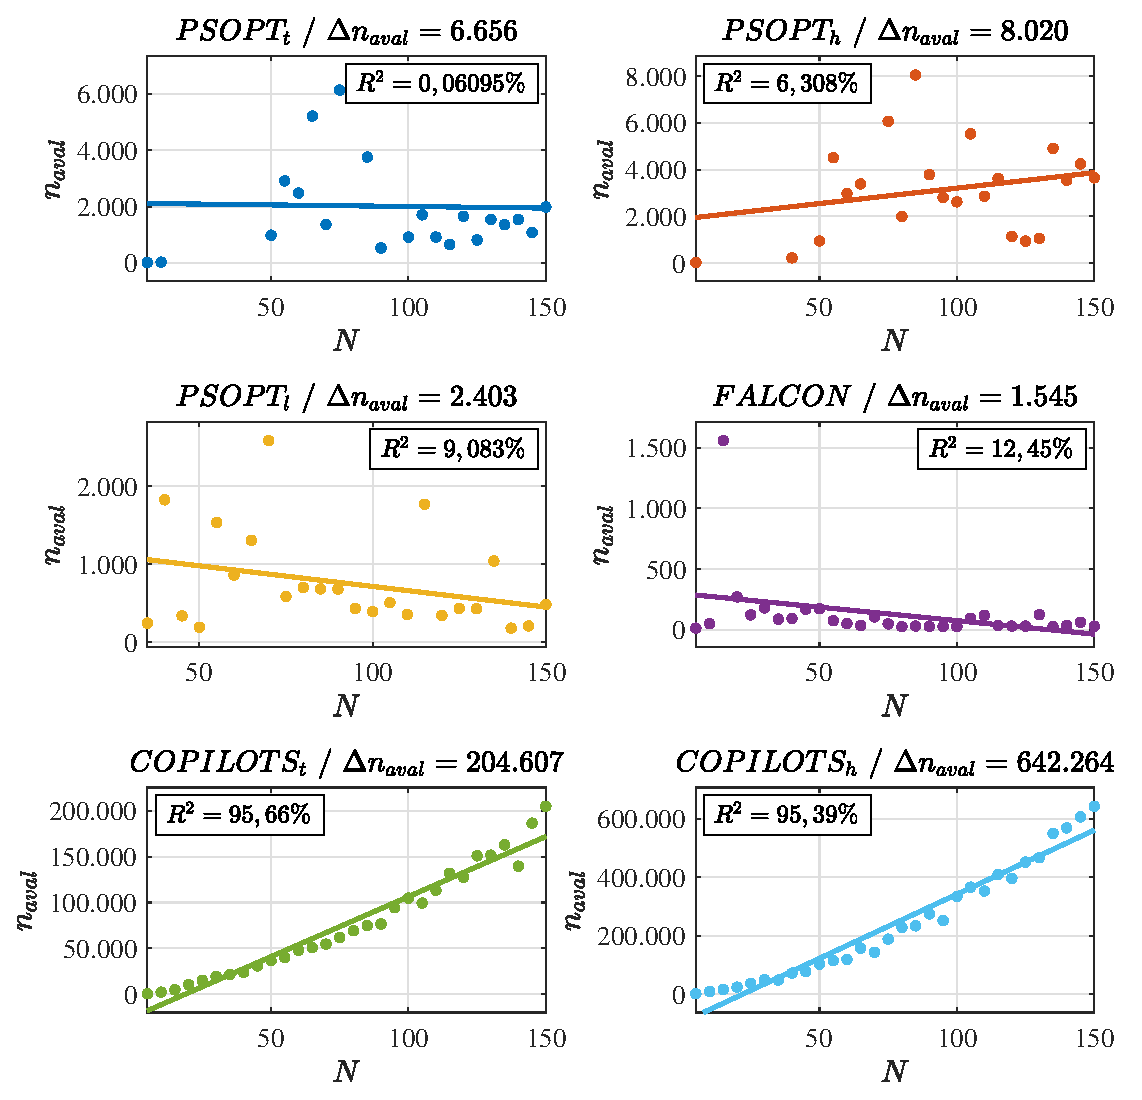
\includegraphics[scale=0.7]{fig/resultados/singular1/sens/eval}
	\captionof{figure}[Relação entre o número de avaliações da função objetivo e o número de nós de colocação para o problema singular 1]{Relação entre o número de avaliações da função objetivo $ n_{aval} $ e o número de nós de colocação $ N $, considerando cada um dos métodos em análise.}
	\label{fig:singular1:sensibilidade:naval}
	\vspace{\onelineskip}
\end{minipage}

